\documentclass[twocolumn,11pt]{article}
\setlength{\textheight}{9truein}
\setlength{\topmargin}{-0.9truein}
\setlength{\parindent}{0pt}
\setlength{\parskip}{10pt}
\setlength{\columnsep}{.4in}

\usepackage{amsmath,amsfonts,amssymb,amsthm,bm,caption,calc,ifthen,graphicx,url,hyperref}

\begin{document}
\pagestyle{plain}
\onecolumn
PHYS689 
\newline Homework 2
\newline Will Wainwright
\newline Repository: \href{https://github.com/wjwainwright/PHYS689}{https://github.com/wjwainwright/PHYS689}

\section*{Gaussian Noise}
For generating Gaussian noise, I used numpy's random.normal() function to generate the noise about a mean with a given standard deviation. I plotted the Gaussian overlay using scipy's normal PDF function given an initial array of evenly spaced x-values. The time series is a plot of the generated values as a function of their index, i.e. the order they were generated. I created a generic function for this process which takes the mean and standard deviation as variables, so changing these values between part 1 and part 2 of the assignment was trivial. I adjusted the number of bins for the normalized histogram manually until I found a number such that the histogram was not too blocky nor too `hairy'. I defined the bin count as a factor of the number of data points n, though n remains constant for this assignment.

\begin{figure}[!h]
	\centering
	\noindent
	\makebox[\textwidth]{
      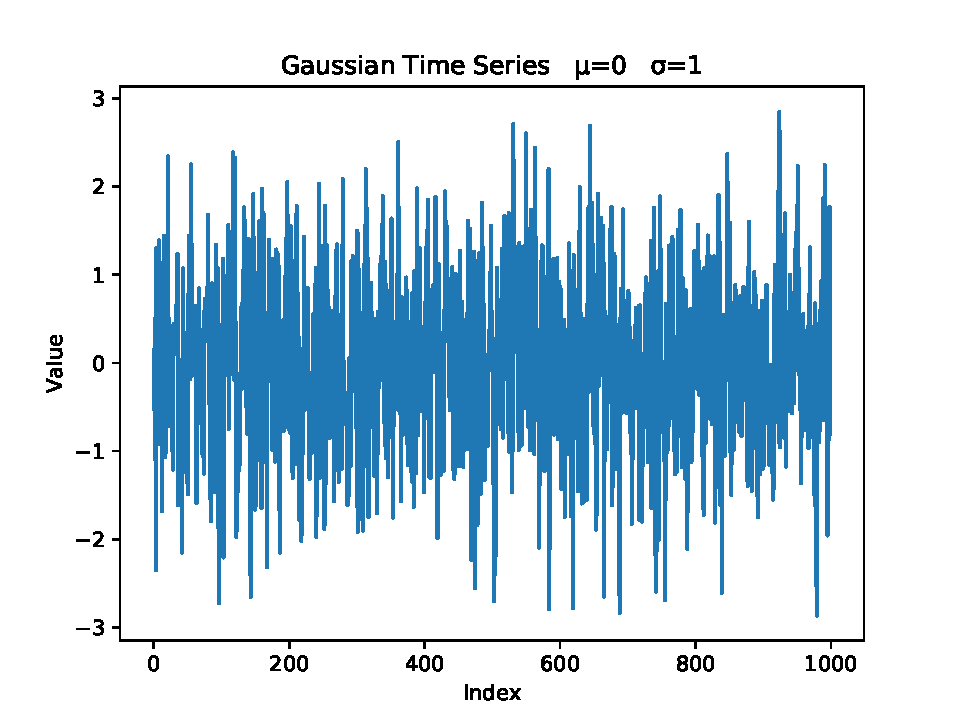
\includegraphics[width=5in]{Gaussian_Timeseries_0_1.pdf}}
      \caption{Gaussian normal distributed time series with $\mu=0$ and $\sigma=1$.}
\end{figure}

\begin{figure}[!h]
	\centering
	\noindent
	\makebox[\textwidth]{
      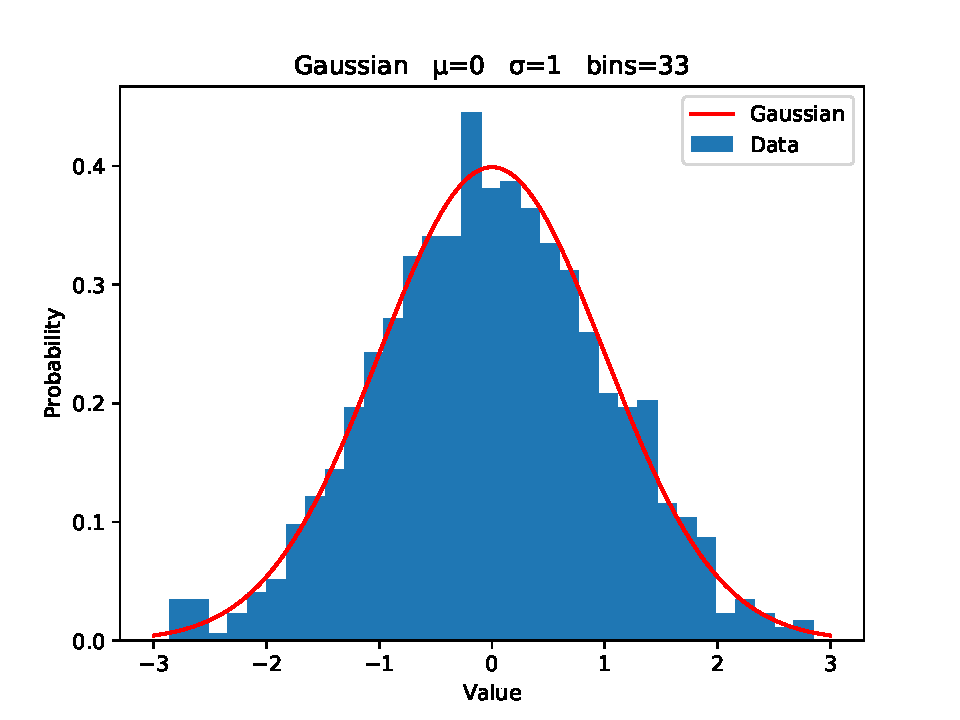
\includegraphics[width=5in]{Gaussian_0_1.pdf}}
      \caption{Gaussian normal distribution histogram with $\mu=0$ and $\sigma=1$.}
\end{figure}

\begin{figure}[!h]
	\centering
	\noindent
	\makebox[\textwidth]{
      \includegraphics[width=5in]{{Gaussian_Timeseries_10.345_2.338}.pdf}}
      \caption{Gaussian normal distributed time series with $\mu=10.345$ and $\sigma=2.338$.}
\end{figure}

\begin{figure}[!h]
	\centering
	\noindent
	\makebox[\textwidth]{
      \includegraphics[width=5in]{{Gaussian_10.345_2.338}.pdf}}
      \caption{Gaussian normal distribution histogram with $\mu=10.345$ and $\sigma=2.338$.}
\end{figure}

\clearpage
\section*{Poisson Noise}
For generating the Poisson noise, I used numpy's random.poisson() function with a given mean. I again plotted a time series of the generated values as a function of index. I plotted a normalized histogram in the same way as before, but for Poisson distribution overlay, I took two different approaches. Depending on the resolution of x values that I defined the Poisson function with, I got either sharp spikes on integer values or a more gradual curve. I found that the sharp spikes were better for identifying the difference between the histogram columns and the expected values. The curve, while less accurate in regards to the value of the function, gives a better view of the expected shape of a continuous or integrated Poisson distribution. For that reason, I decided to keep both types of plots and labeled them `Sharp' and `Fuzzy' accordingly. 

\begin{figure}[!h]
	\centering
	\noindent
	\makebox[\textwidth]{
      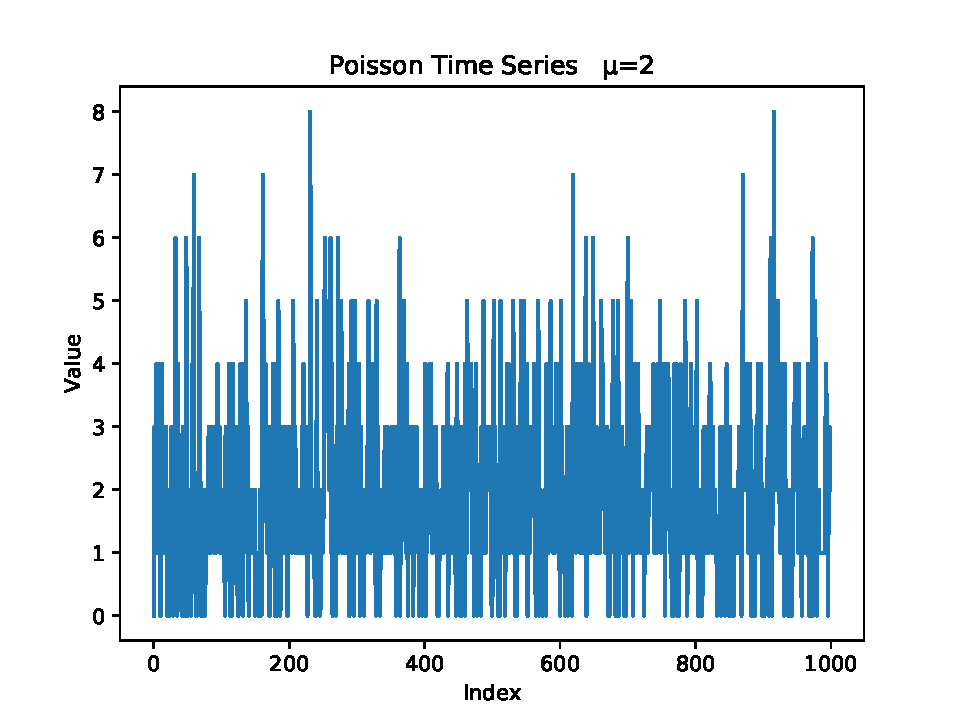
\includegraphics[width=5in]{Poisson_Timeseries_2.pdf}}
      \caption{Poisson distributed time series with $\mu=2$.}
\end{figure}

\begin{figure}[!h]
	\centering
	\noindent
	\makebox[\textwidth]{
      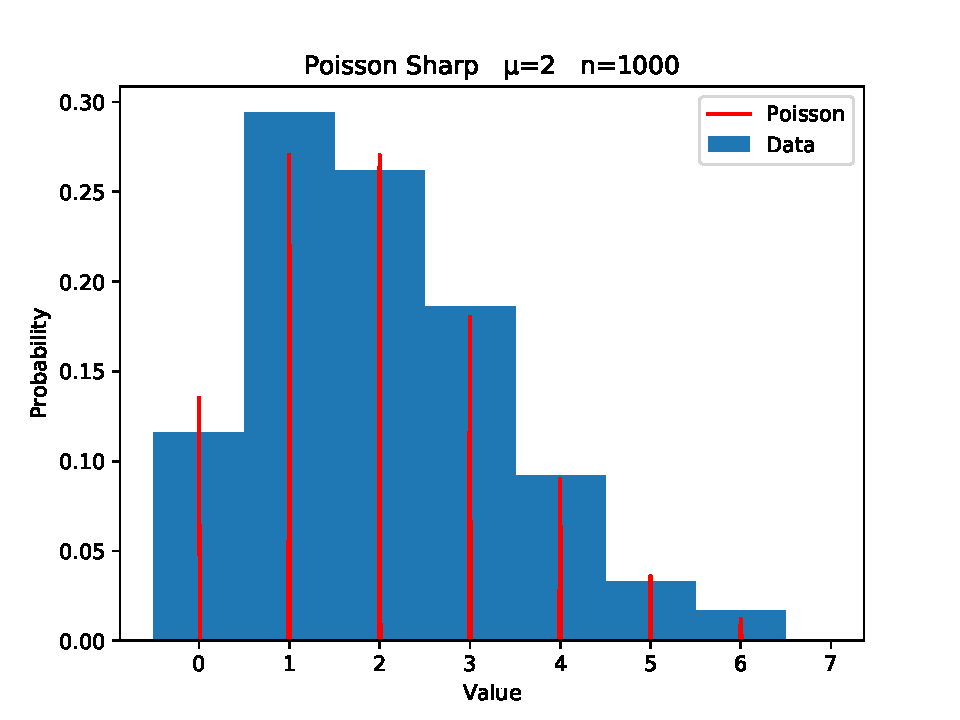
\includegraphics[width=5in]{Poisson_Sharp_2.pdf}}
      \caption{Poisson distribution histogram with $\mu=2$. The PDF peaks sharply as it is defined with a high resolution.}
\end{figure}

\begin{figure}[!h]
	\centering
	\noindent
	\makebox[\textwidth]{
      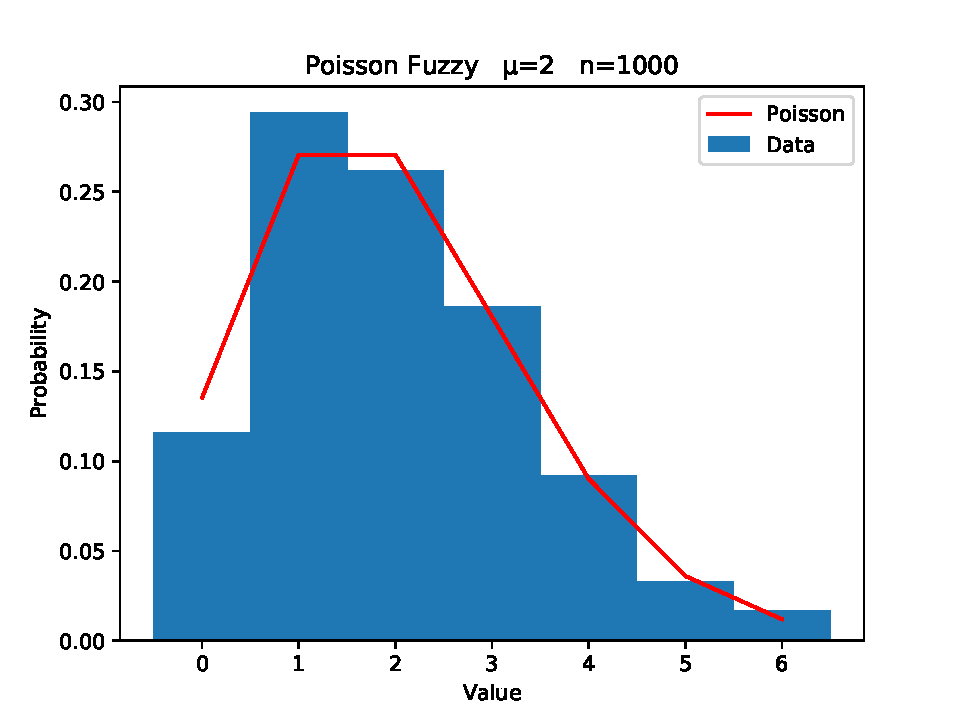
\includegraphics[width=5in]{Poisson_Fuzzy_2.pdf}}
      \caption{Poisson distribution histogram with $\mu=2$. The PDF peaks gradually as it is defined with a low resolution.}
\end{figure}

\begin{figure}[!h]
	\centering
	\noindent
	\makebox[\textwidth]{
      \includegraphics[width=5in]{{Poisson_Timeseries_3.45}.pdf}}
      \caption{Poisson distributed time series with $\mu=3.45$.}
\end{figure}

\begin{figure}[!h]
	\centering
	\noindent
	\makebox[\textwidth]{
      \includegraphics[width=5in]{{Poisson_Sharp_3.45}.pdf}}
      \caption{Poisson distribution histogram with $\mu=3.45$. The PDF peaks sharply as it is defined with a high resolution.}
\end{figure}

\begin{figure}[!h]
	\centering
	\noindent
	\makebox[\textwidth]{
      \includegraphics[width=5in]{{Poisson_Fuzzy_3.45}.pdf}}
      \caption{Poisson distribution histogram with $\mu=3.45$. The PDF peaks gradually as it is defined with a low resolution.}
\end{figure}

\end{document}